
\chapter{演奏と録音}

\section{初演から出版まで}\label{sec: till publication}

出版までに本作は手稿譜の状態で次の都市で演奏された. 英国で演奏されているのは,
ケンブリッジ大学から名誉博士号を授与されるために渡英したJoachimにBrahmsが手稿譜を託したためである\cite{kaisouroku}. 
\begin{quote}
\begin{multicols}{2}
	\begin{itemize}
		\item カールスルーエ (11/4)
		\item マンハイム (11/7)
		\item ミュンヘン (11/15)
		\item ウィーン (12/17)
		\item ライプツィヒ (1/18)
		\item ブレスラウ (1/23)
		\item ケンブリッジ (3/7)
		\item ロンドン (3/31, 4/16)
	\end{itemize}
\end{multicols}
\end{quote}

\begin{figure}[htbp]
	\begin{center}
    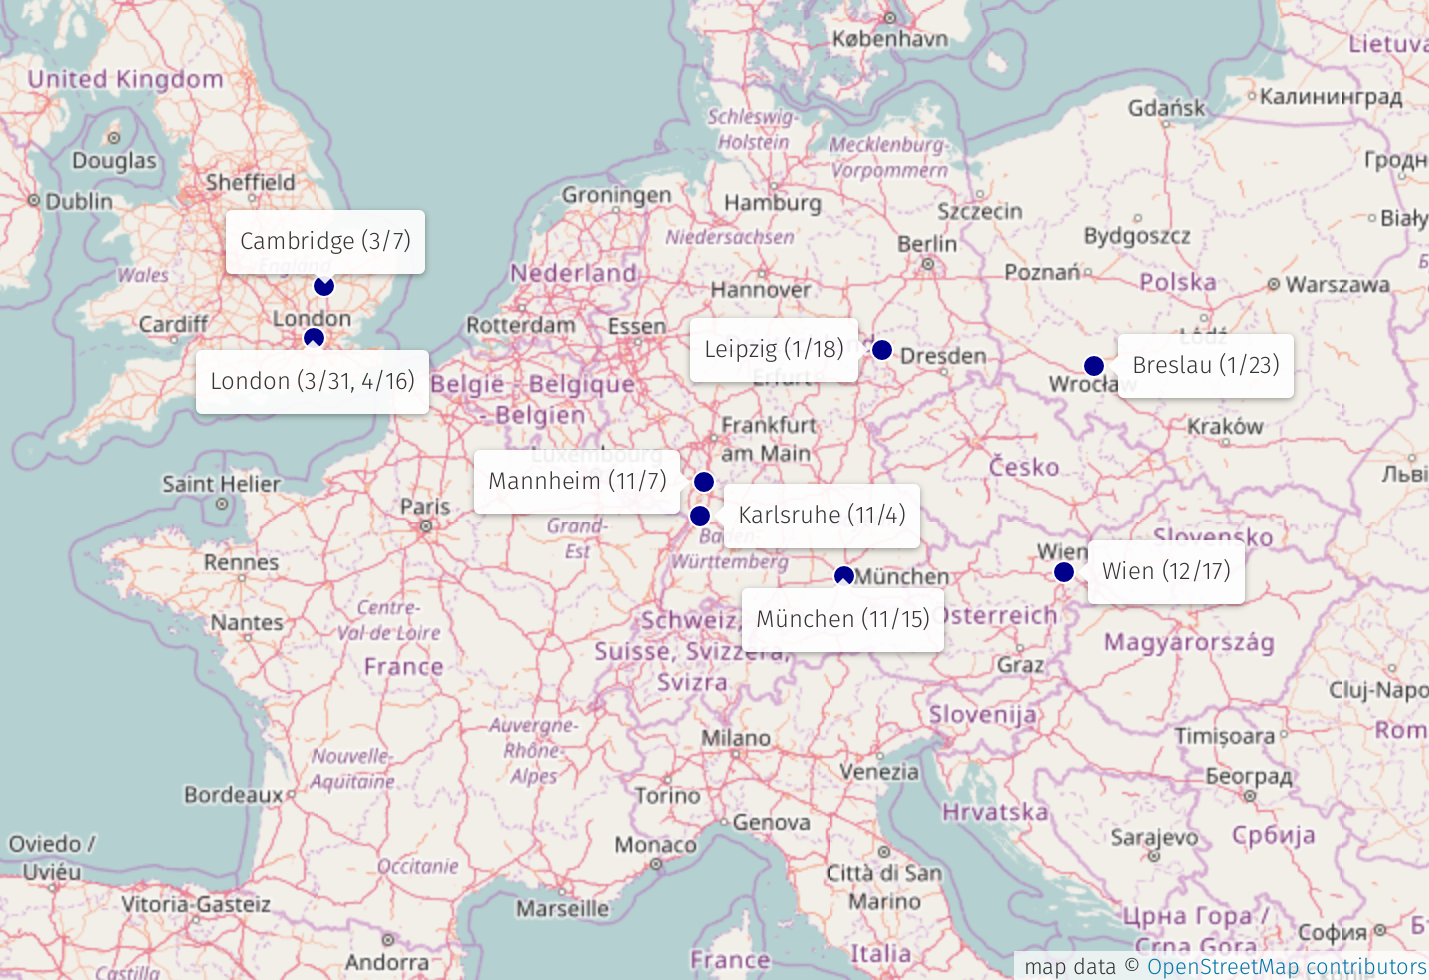
\includegraphics[clip,width=14.0cm]{./figure/map-concert.png}
	\caption{交響曲第1番が手稿譜で演奏された都市.
		地図はOpenStreetMapによる (\href{http://www.openstreetmap.org/copyright}{CC BY-SA}).}
    \label{fig: concert}
	\end{center}
\end{figure}

\section{19世紀ドイツ・オーストリアにおける受容}

\section{ヨーロッパおよびアメリカ}

\section{日本における演奏史}

\section{録音}

% この傑作の録音の完全なリストを作成することは (演奏のリストほどではないにしても) 到底実現不可能である.
% なんらかの基準を設けて項目を選択したとしても, その基準の妥当性が問題になる.
% 従ってここに掲載するリストは筆者の独断と偏見を多分に含むことになる.
